% ==============================================================================
% SECTION 3: BAROTRAUMATISMES
% ==============================================================================
\section{Les Barotraumatismes}

\begin{frame}{Définition et Généralités}
    \begin{block}{Rappels}
        En plongée, les volumes de gaz sont inversement proportionnels à la pression qu'ils subissent.
    \end{block}

    \vspace{0.3cm}

    \textbf{Définition :} Résultat du non-équilibre entre un volume gazeux du corps et la pression ambiante.
    
    \begin{itemize}
        \item \textbf{Facteur favorisant :} Variation RAPIDE de pression.
        \item \textbf{Zone à risque :} Proche de la surface (variations de volume importantes).
    \end{itemize}
    
    \textit{Le N3 doit savoir prévenir et gérer l'accident en l'absence de DP.}

    \vspace{0.4cm}
    
    \begin{block}{Résumé}
        Ils se caractérisent par leur effet immédiat et un facteur favorisant commun : une variation \textbf{rapide} de pression.
    \end{block}
\end{frame}

\begin{frame}{Attentes pédagogiques N3 — Barotraumatismes}
    Le plongeur Niveau 3 doit connaître les différents accidents barotraumatiques.\\
    Pour chacun d'eux, il doit :
    \begin{itemize}
        \item connaître la cause
        \item connaître les symptômes permettant de les détecter
        \item savoir les prévenir
        \item connaître l'ensemble de la conduite à tenir (CAT)
        \item être capable de répondre à des questions écrites ou orales en vue de l'examen
    \end{itemize}
\end{frame}

\begin{frame}{Surpression Pulmonaire — Schéma}
    \begin{columns}
        \column{0.7\textwidth}
        \centering
        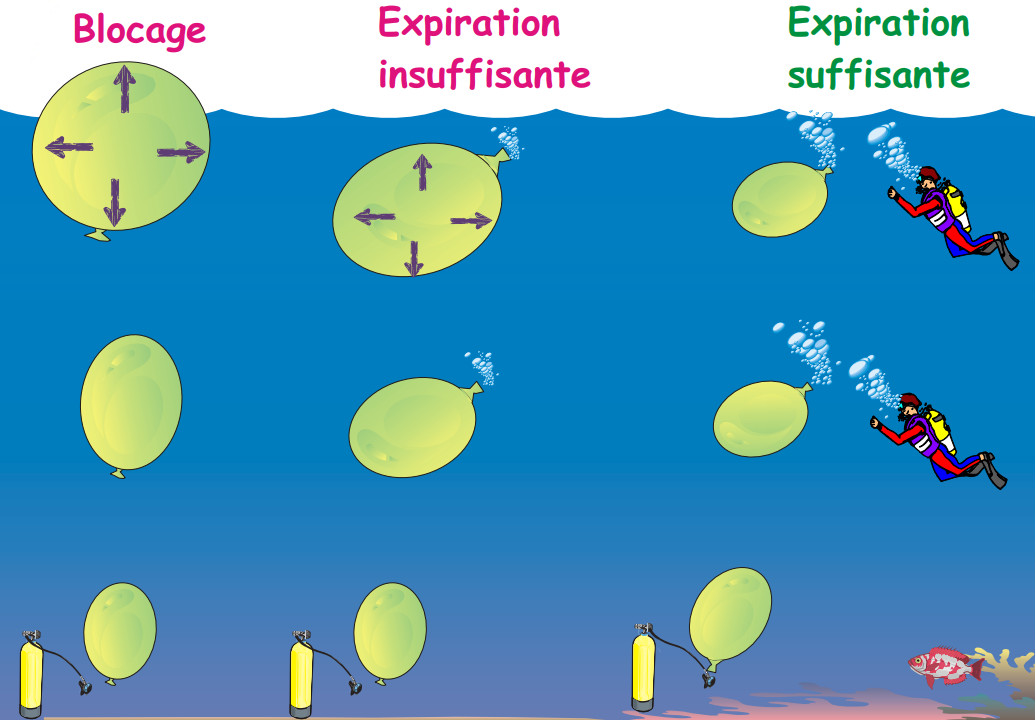
\includegraphics[height=0.85\textheight]{images/surpression_pulmonaire.png}

        \column{0.3\textwidth}
        \centering
        \small Schéma illustrant la surpression pulmonaire et l'expansion des gaz à la remontée.
    \end{columns}
\end{frame}

\begin{frame}{Surpression Pulmonaire — Conséquences}
    \begin{columns}
        \column{0.6\textwidth}
        \centering
        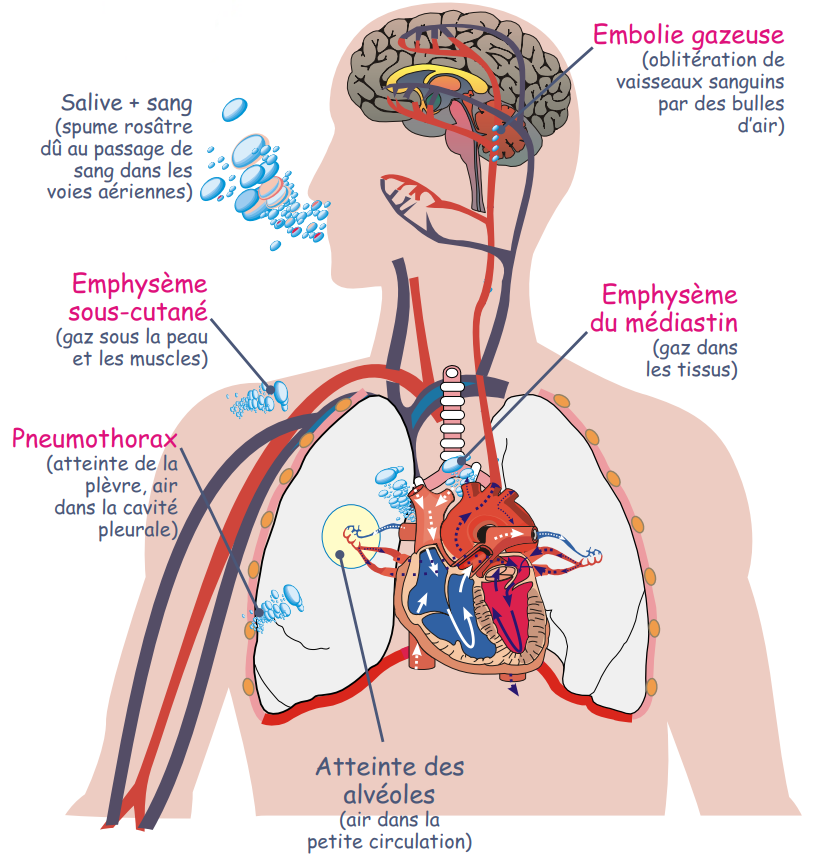
\includegraphics[height=0.85\textheight]{images/surpression_pulmonaire_consequences.png}

        \column{0.4\textwidth}
        \centering
        \small Principales conséquences de la surpression pulmonaire (embolie, emphysème, etc.).
    \end{columns}
\end{frame}

\begin{frame}{Surpression Pulmonaire - Résumé}
    \textbf{Cause :} Augmentation du volume pulmonaire au-delà de la tolérance (blocage respiration).
    
    \textbf{Symptômes :}
    \begin{itemize}
        \item Douleurs thoraciques.
        \item Difficultés respiratoires, crachats sanglants.
        \item Peut être fatal rapidement.
    \end{itemize}
    
    \textbf{Prévention N3 :}
    \begin{itemize}
        \item Gérer sa vitesse de remontée (ordinateur, bulles).
        \item Expiration continue à la remontée.
    \end{itemize}
\end{frame}

\begin{frame}{Surpression Pulmonaire — Conduite à Tenir (CAT)}
    \begin{columns}[T,totalwidth=\textwidth]
        \column{0.55\textwidth}
        \begin{itemize}
            \item \textbf{\textcolor{ffessmred}{Position}} confortable: \textbf{\textcolor{ffessmred}{demi-assise}} ou \textbf{\textcolor{ffessmred}{allongée}}.
            \item \textbf{\textcolor{ffessmred}{Déséquiper}} (bloc, stab, combi).
            \item \textbf{\textcolor{ffessmred}{Oxygène}}: \textbf{\textcolor{ffessmred}{15 L/min}} (masque haute concentration).
        \end{itemize}

        \column{0.45\textwidth}
        \begin{itemize}
            \item Si \textbf{\textcolor{ffessmred}{consciente}}: petites gorgées \textbf{\textcolor{ffessmred}{d'eau}}.
            \item \textbf{\textcolor{ffessmred}{Alerter}} les secours.
            \item \textbf{\textcolor{ffessmred}{Évacuation rapide}} (prise en charge type \textbf{\textcolor{ffessmred}{ADD}}).
        \end{itemize}
    \end{columns}
\end{frame}

\begin{frame}{Barotraumatisme de l'Oreille — Descente}
    \begin{columns}[T,totalwidth=\textwidth]
        \column{0.55\textwidth}
        \centering
        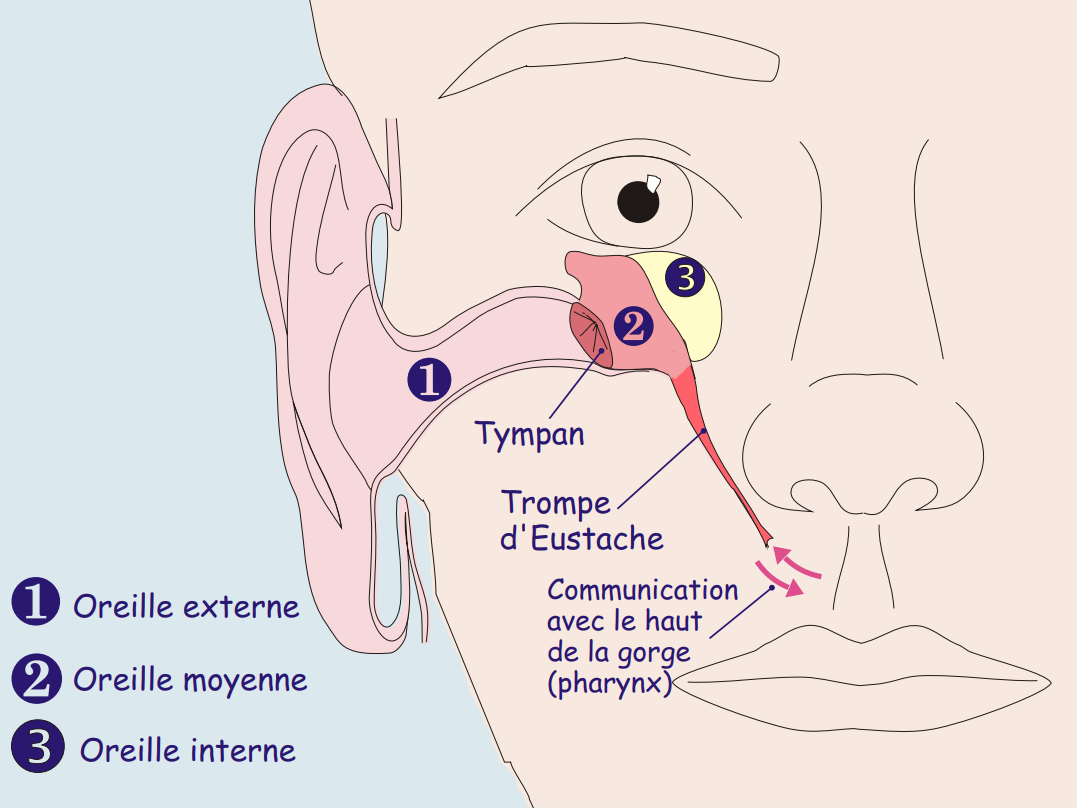
\includegraphics[height=0.8\textheight]{images/baro_oreille.png}

        \column{0.4\textwidth}
        \small
        \textbf{\textcolor{ffessmred}{Équilibrage}} régulier à la descente (Valsalva, déglutition).\\[0.5em]
        \textbf{Descente (Oreille moyenne)}
        \begin{itemize}
            \item \textit{Cause} : Non-équilibrage ou Valsalva tardif.
            \item \textit{Symptôme} : \textbf{\textcolor{ffessmred}{douleur aiguë}}.
            \item \textit{Prévention} : manœuvres \textbf{\textcolor{ffessmred}{douces et précoces}}, ne pas forcer.
            \item \textbf{\textcolor{ffessmred}{CAT}} : stopper la descente, corriger l'équilibrage.
        \end{itemize}

        \begin{alertblock}{Attention — \textbf{Coup de piston}}
            Forcer la \textbf{\textcolor{ffessmred}{Valsalva}} = surpression brutale
        \end{alertblock}
    \end{columns}
\end{frame}

\begin{frame}{Barotraumatisme de l'Oreille — Remontée}
    \begin{columns}[T,totalwidth=\textwidth]
        \column{0.55\textwidth}
        \centering
        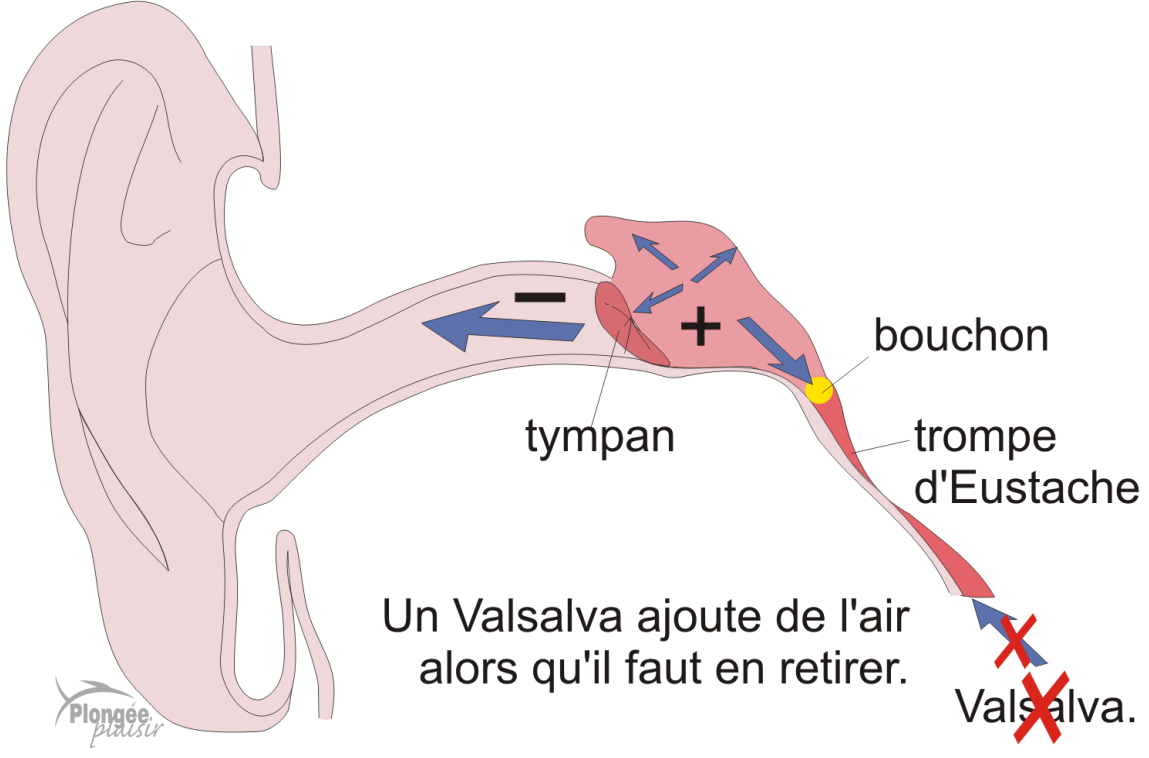
\includegraphics[height=0.7\textheight]{images/baro_oreille_vertige_alterno_barique.png}

        \column{0.4\textwidth}
        \small
        \textbf{Remontée (Vertige alterno-barique)}
        \begin{itemize}
            \item \textit{Cause} : Une oreille s'équilibre mal (bouchon, mucosité).
            \item \textit{Symptôme} : \textbf{\textcolor{ffessmred}{vertiges intenses}} à la remontée.
            \item \textit{Action} : \textbf{\textcolor{ffessmred}{redescendre un peu}}, déglutir, \textbf{\textcolor{ffessmred}{remonter lentement}}.
            \item \textbf{\textcolor{ffessmred}{Prévention}} : hygiène ORL, éviter de plonger enrhumé.
        \end{itemize}
        \begin{alertblock}{Attention — \textbf{Pas de Valsalva}}
            \textbf{\textcolor{ffessmred}{Valsalva}} = Surpression pulmonaire
        \end{alertblock}
    \end{columns}
\end{frame}

\begin{frame}{Vertige alterno-barique — \textbf{Symptômes} et \textbf{CAT}}
    \textbf{Symptômes} :
    \begin{itemize}
        \item Apparaissent \textbf{\textcolor{ffessmred}{sous l'eau}} pendant la \textbf{\textcolor{ffessmred}{remontée}} (différencier d'un \textbf{ADD} souvent \textbf{\textcolor{ffessmred}{à la sortie}}).
        \item \textbf{\textcolor{ffessmred}{Vertiges}} fugaces ou durables, parfois \textbf{\textcolor{ffessmred}{nausées}}.
        \item S'atténuent et \textbf{\textcolor{ffessmred}{disparaissent}} en quelques minutes après le retour à la surface.
    \end{itemize}

    \vspace{0.5em}
    \textbf{Conduite à Tenir (CAT)} :
    \begin{itemize}
        \item Maintenir une \textbf{\textcolor{ffessmred}{vigilance}} auprès du \textbf{\textcolor{ffessmred}{binôme}}.
        \item Conseiller une \textbf{\textcolor{ffessmred}{consultation ORL}} si \textbf{\textcolor{ffessmred}{douleur persistante}} à la sortie de l'eau.
    \end{itemize}
\end{frame}

\begin{frame}{Barotraumatisme des Sinus — Causes \& Mécanismes}
    \begin{columns}[T,totalwidth=\textwidth]
        \column{0.55\textwidth}
        \centering
        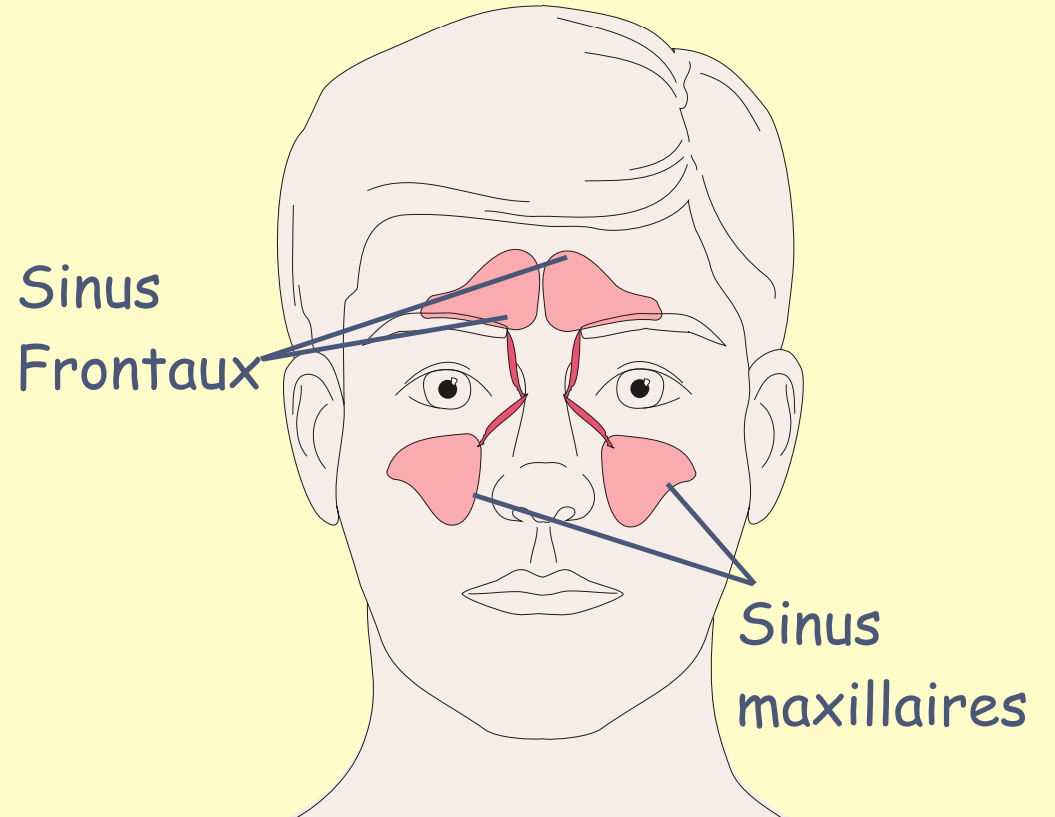
\includegraphics[height=0.75\textheight]{images/baro_sinus.png}

        \column{0.45\textwidth}
        \small
        Causes :
        \begin{itemize}
            \item Cavités de la face tapissées de \textbf{\textcolor{ffessmred}{muqueuse}}.
            \item \textbf{\textcolor{ffessmred}{Non-équilibre}} des sinus à la \textbf{descente} et à la \textbf{remontée}.
        \end{itemize}

        \vspace{0.4em}
        Mécanismes :
        \begin{itemize}
            \item \textbf{\textcolor{ffessmred}{Œdème / déformation}} de la muqueuse.
            \item \textbf{\textcolor{ffessmred}{Obstruction}} des ostia empêchant l'\textbf{\textcolor{ffessmred}{équilibrage}}.
        \end{itemize}
    \end{columns}
\end{frame}

\begin{frame}{Barotraumatisme des Sinus — Facteurs favorisants}
    \begin{block}{\textbf{Facteurs favorisants}}
        \begin{itemize}
            \item \textbf{\textcolor{ffessmred}{Vitesse}} de descente/remontée trop \textbf{\textcolor{ffessmred}{rapide}} si équilibrage difficile.
            \item En autonomie: adapter la \textbf{\textcolor{ffessmred}{vitesse}} pour tous; garder le \textbf{\textcolor{ffessmred}{dialogue}} binôme.
            \item \textbf{\textcolor{ffessmred}{Vasoconstricteurs}} déconseillés (effet court) → \textbf{\textcolor{ffessmred}{soucis d'équilibrage}} à la remontée.
        \end{itemize}
    \end{block}
\end{frame}

\begin{frame}{Barotraumatisme des Sinus — Symptômes \& CAT}
    Symptômes :
    \begin{itemize}
        \item Sinus \textbf{\textcolor{ffessmred}{encombrés}} (allergie, \textbf{\textcolor{ffessmred}{rhume}}) → air s'infiltre mal.
        \item \textbf{\textcolor{ffessmred}{Douleur faciale}} type « coup de poignard », parfois épistaxis (saignement de nez).
        \item Difficulté à s'\textbf{\textcolor{ffessmred}{équilibrer}} comme les fosses nasales.
    \end{itemize}

    \vspace{0.5em}
    Conduite à Tenir (CAT) :
    \begin{itemize}
        \item \textbf{\textcolor{ffessmred}{Ne pas faire}} d'équilibrage; \textbf{\textcolor{ffessmred}{stopper}} et \textbf{\textcolor{ffessmred}{ralentir}} la progression.
        \item \textbf{\textcolor{ffessmred}{Rincer}} les fosses nasales à l'eau de mer pour faciliter le passage de l'air.
        \item \textbf{\textcolor{ffessmred}{Ne pas plonger}} enrhumé; hygiène ORL.
        \item Consulter/demander un \textbf{\textcolor{ffessmred}{avis médical}} si gêne ou \textbf{\textcolor{ffessmred}{douleur persistante}} à la sortie de l'eau.
    \end{itemize}
\end{frame}

\begin{frame}{Placage de masque — Causes, Mécanismes}
    \begin{columns}[T,totalwidth=\textwidth]
        \column{0.55\textwidth}
        \centering
        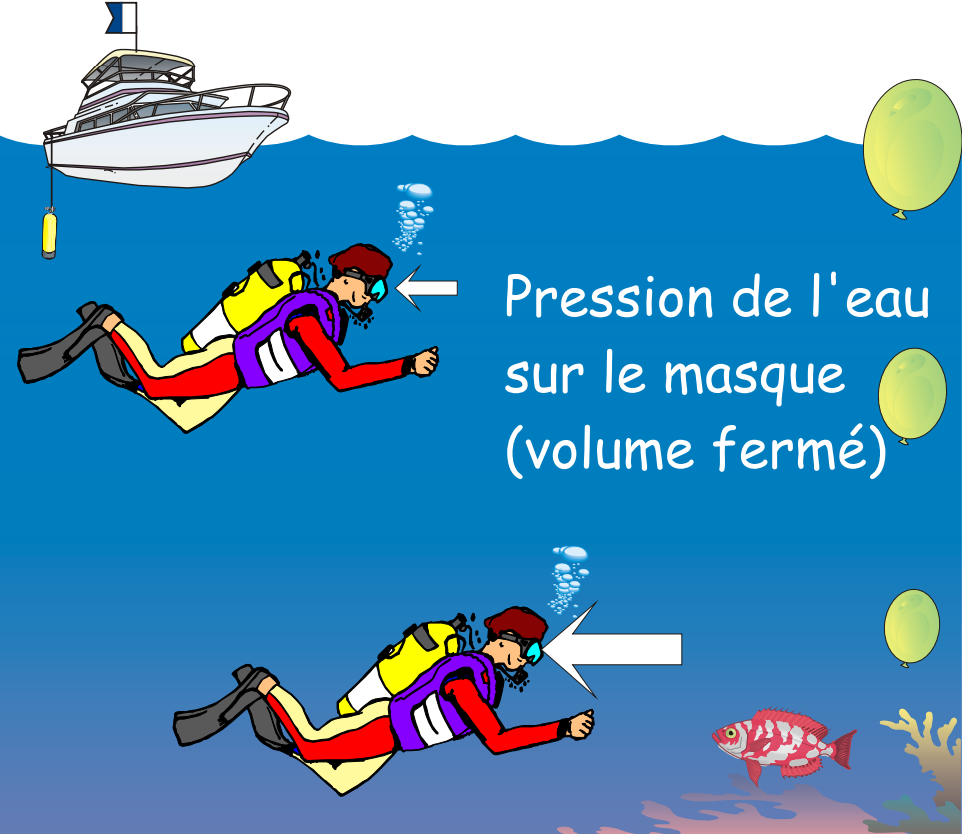
\includegraphics[height=0.75\textheight]{images/baro_masque.png}

        \column{0.45\textwidth}
        Cause :
        \begin{itemize}
            \item À la \textbf{descente}, \textbf{\textcolor{ffessmred}{non-équilibre}} du volume d'air du masque avec le milieu ambiant.
        \end{itemize}

        \vspace{0.3em}
        Mécanismes :
        \begin{itemize}
            \item \textbf{\textcolor{ffessmred}{Effet ventouse}} sur le visage.
            \item Le volume d'air entre la face et la vitre \textbf{varie} avec la \textbf{pression}.
            \item Avec l'\textbf{augmentation de pression}, le masque se \textbf{\textcolor{ffessmred}{plaque}} sur le visage.
        \end{itemize}
    \end{columns}
\end{frame}

\begin{frame}{Placage de masque — Symptômes, CAT}
    \vspace{0.3em}
    Facteurs favorisants :
    \begin{itemize}
        \item \textbf{\textcolor{ffessmred}{Sangle trop serrée}} (moins d'élasticité de la jupe).
        \item \textbf{\textcolor{ffessmred}{Vitesse}} de descente \textbf{rapide}.
    \end{itemize}

    \vspace{0.3em}
    Symptômes :
    \begin{itemize}
        \item Troubles de la \textbf{\textcolor{ffessmred}{vue}}, lésions légères \textbf{yeux/nez} (non graves, non irréversibles).
    \end{itemize}

    \vspace{0.3em}
    Conduite à Tenir (CAT) :
    \begin{itemize}
        \item \textbf{\textcolor{ffessmred}{Souffler par le nez}} à la descente pour \textbf{\textcolor{ffessmred}{équilibrer}} le masque.
        \item \textbf{\textcolor{ffessmred}{Adapter}} la vitesse et \textbf{\textcolor{ffessmred}{desserrer}} légèrement la sangle si besoin.
        \item \textbf{\textcolor{ffessmred}{Avis médical}} si gêne/douleur \textbf{\textcolor{ffessmred}{persistante}} à la sortie de l'eau.
    \end{itemize}
\end{frame}

\begin{frame}{Autres Barotraumatismes}
    \begin{itemize}
        \item \textbf{\textcolor{ffessmred}{Estomac/Intestin}} :
        \begin{itemize}
            \item Accident \textbf{rare} chez le plongeur actuel; concernait surtout les \textbf{scaphandriers « pieds lourds »} (alimentation abondante).
            \item Gaz digestifs qui se \textbf{dilatent} à la remontée → gêne/douleur.
            \item \textbf{Prévention/CAT} : éviter repas lourds avant plongée, \textbf{ralentir} si gêne, \textbf{évacuer l'air} si possible.
        \end{itemize}

        \vspace{0.4em}
        \item \textbf{\textcolor{ffessmred}{Dents}} :
        \begin{itemize}
            \item \textbf{Descente} : gencives \textbf{fragiles} plus sensibles (pression, froid de l'air détendu) → \textbf{remonter} et \textbf{stopper}.
            \item \textbf{Remontée} : poche d'air sous \textbf{dent cariée/mal soignée} → \textbf{douleur croissante}.
            \item \textbf{Prévention} : \textbf{bonne hygiène dentaire}.
            \item \textbf{CAT} : \textbf{stopper} la progression; si douleur, \textbf{redescendre 1–2 m} puis \textbf{remonter lentement}; \textbf{consulter} si douleur persistante.
        \end{itemize}
    \end{itemize}
\end{frame}

\begin{frame}{Synthèse des Barotraumatismes}
    \centering
    \renewcommand{\arraystretch}{1.4} % Aère le tableau
    \footnotesize % Réduit légèrement la police pour que tout rentre
    
    \begin{table}[]
        \begin{tabular}{p{2cm} c p{3.5cm} p{3.5cm}}
        \toprule
        \textbf{Type} & \textbf{Qd?} & \textbf{Prévention Clé} & \textbf{Conduite à Tenir (CAT)} \\ 
        \midrule
        
        \textbf{Surpression Pulmonaire} & $\nearrow$ & 
        Expiration continue \newline Vitesse contrôlée & 
        \textbf{Urgence Vitale !} \newline O2 (15L/min) + Évacuation \\ 
        \hline
        
        \textbf{Oreilles \newline \& Sinus} & $\searrow$ \newline $\nearrow$ & 
        Manœuvres douces \newline Ne jamais forcer \newline Vitesse lente & 
        Stopper l'immersion \newline Consulter ORL si douleur persistante \\ 
        \hline
        
        \textbf{Dents} & $\searrow \nearrow$ & 
        Hygiène dentaire \newline Stop si douleur & 
        Consultation dentiste \\ 
        \hline
        
        \textbf{Masque} & $\searrow$ & 
        Souffler par le nez & 
        - \\ 
        \hline
        
        \textbf{Intestins} & $\nearrow$ & 
        Alimentation saine \newline Évacuer les gaz & 
        Consultation si douleur \\ 
        
        \bottomrule
        \end{tabular}
    \end{table}

    \vspace{0.2cm}
    \scriptsize{Légende : $\searrow$ Descente \quad $\nearrow$ Remontée}
\end{frame}